\documentclass{standalone}
\usepackage[dvipsnames,svgnames,x11names]{xcolor}
\usepackage{tikz}
\usepackage{pgfplots}
\usetikzlibrary{pgfplots.statistics}
\pgfplotsset{compat = 1.12}
\usepackage[
  group-separator={,},
  exponent-product=\cdot,
]{siunitx}
\usepackage{../thesismath}
\begin{document}
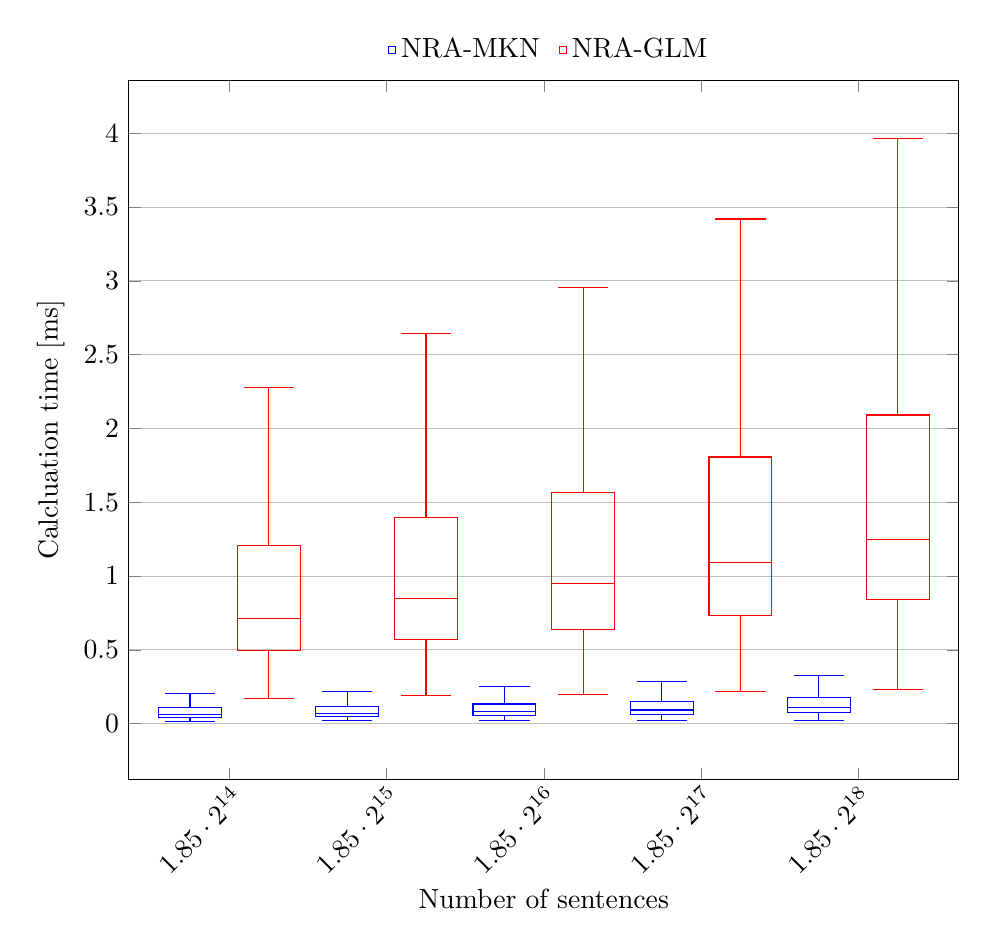
\begin{tikzpicture}[baseline]

\pgfplotscreateplotcyclelist{mkn_glm}{%
  blue,  mark size=1.25, mark=square,\\%
  red,   mark size=1.25, mark=square,\\%
}

\pgfplotsset{
  legend style = {
    draw = none,
    legend image code/.code = {
      \draw[only marks]
        plot coordinates {
          (0.3cm,0cm)
        };
      \node at (0.15cm, 0cm) {};
    },
  },
  boxplot/draw/average/.code = {
    %% uncomment to show dotted bars for average:
    %\draw[dashed, /pgfplots/boxplot/every average/.try]
    %  (boxplot box cs:\pgfplotsboxplotvalue{average},0)
    %  --
    %  (boxplot box cs:\pgfplotsboxplotvalue{average},1)
    %  ;
  },
}

\sisetup{exponent-base = 2}
\begin{axis}[
  xlabel = {Number of sentences},
  xtick       = {            1,             2,             3,             4,             5},
  xticklabels = {\num{1.85e14}, \num{1.85e15}, \num{1.85e16}, \num{1.85e17}, \num{1.85e18}},
  xticklabel style={
    inner sep = 1pt,
    anchor = north east,
    rotate = 45,
  },
  ylabel = {Calcluation time [\si{\milli\second}]},
  scaled y ticks = false,
  log ticks with fixed point,
  boxplot/draw direction = y,
  cycle list name = mkn_glm,
  grid = major,
  xmajorgrids = false,
  legend entries = {{NRA-MKN}, {NRA-GLM}},
  legend style = {
    anchor=south,
    at={(axis description cs: 0.5, 1.01)}
  },
  legend columns = 3,
  width = \textwidth,
]

% training-5-argmaxcompare-40k-c/ngram-5-NRA-Weighted-Sum-Modified-Kneser-Ney-1
\addplot+[
  boxplot prepared = {
    %draw position = 30400,
    draw position = 1,
    box extend = 0.4,
    lower whisker = 0.017407,
    lower quartile = 0.042866,
    median = 0.063964,
    upper quartile = 0.108526,
    upper whisker = 0.207005,
    average = 0.367642,
  },
  xshift = -0.5cm,
] table [row sep = \\, y index = 0] {
  data\\
};

% training-5-argmaxcompare-40k-c/ngram-5-NRA-Weighted-Sum-Generalized-Language-Model-1
\addplot+[
  boxplot prepared = {
    %draw position = 30400,
    draw position = 1,
    box extend = 0.4,
    lower whisker = 0.172192,
    lower quartile = 0.492755,
    median = 0.714188,
    upper quartile = 1.206376,
    upper whisker = 2.276287,
    average = 1.227375,
  },
  xshift = 0.5cm,
] table [row sep = \\, y index = 0] {
  data\\
};

% ------------------------------------------------------------------------------

% training-4-argmaxcompare-40k-c/ngram-5-NRA-Weighted-Sum-Modified-Kneser-Ney-1
\addplot+[
  boxplot prepared = {
    %draw position = 60801,
    draw position = 2,
    box extend = 0.4,
    lower whisker = 0.019593,
    lower quartile = 0.049044,
    median = 0.071640,
    upper quartile = 0.117478,
    upper whisker = 0.220049,
    average = 0.463580,
  },
  xshift = -0.5cm,
] table [row sep = \\, y index = 0] {
  data\\
};

% training-4-argmaxcompare-40k-c/ngram-5-NRA-Weighted-Sum-Generalized-Language-Model-1
\addplot+[
  boxplot prepared = {
    %draw position = 60801,
    draw position = 2,
    box extend = 0.4,
    lower whisker = 0.191494,
    lower quartile = 0.571501,
    median = 0.845661,
    upper quartile = 1.399696,
    upper whisker = 2.641562,
    average = 1.422414,
  },
  xshift = 0.5cm,
] table [row sep = \\, y index = 0] {
  data\\
};


% ------------------------------------------------------------------------------

% training-3-argmaxcompare-40k-c/ngram-5-NRA-Weighted-Sum-Modified-Kneser-Ney-1
\addplot+[
  boxplot prepared = {
    %draw position = 121602,
    draw position = 3,
    box extend = 0.4,
    lower whisker = 0.020295,
    lower quartile = 0.054553,
    median = 0.080047,
    upper quartile = 0.132983,
    upper whisker = 0.250549,
    average = 0.441277,
  },
  xshift = -0.5cm,
] table [row sep = \\, y index = 0] {
  data\\
};

% training-3-argmaxcompare-40k-c/ngram-5-NRA-Weighted-Sum-Generalized-Language-Model-1
\addplot+[
  boxplot prepared = {
    %draw position = 121602,
    draw position = 3,
    box extend = 0.4,
    lower whisker = 0.200491,
    lower quartile = 0.636782,
    median = 0.951191,
    upper quartile = 1.564153,
    upper whisker = 2.954344,
    average = 1.641707,
  },
  xshift = 0.5cm,
] table [row sep = \\, y index = 0] {
  data\\
};

% ------------------------------------------------------------------------------

% training-2-argmaxcompare-40k-c/ngram-5-NRA-Weighted-Sum-Modified-Kneser-Ney-1
\addplot+[
  boxplot prepared = {
    %draw position = 2432004,
    draw position = 4,
    box extend = 0.4,
    lower whisker = 0.019813,
    lower quartile = 0.062182,
    median = 0.092578,
    upper quartile = 0.150630,
    upper whisker = 0.283221,
    average = 0.553668,
  },
  xshift = -0.5cm,
] table [row sep = \\, y index = 0] {
  data\\
};

% training-2-argmaxcompare-40k-c/ngram-5-NRA-Weighted-Sum-Generalized-Language-Model-1
\addplot+[
  boxplot prepared = {
    %draw position = 2432004,
    draw position = 4,
    box extend = 0.4,
    lower whisker = 0.219336,
    lower quartile = 0.731608,
    median = 1.094962,
    upper quartile = 1.806765,
    upper whisker = 3.418836,
    average = 1.912399,
  },
  xshift = 0.5cm,
] table [row sep = \\, y index = 0] {
  data\\
};

% ------------------------------------------------------------------------------

% training-1-argmaxcompare-40k-c/ngram-5-NRA-Weighted-Sum-Modified-Kneser-Ney-1
\addplot+[
  boxplot prepared = {
    %draw position = 486409,
    draw position = 5,
    box extend = 0.4,
    lower whisker = 0.023497,
    lower quartile = 0.073006,
    median = 0.110507,
    upper quartile = 0.174697,
    upper whisker = 0.327149,
    average = 0.608050,
  },
  xshift = -0.5cm,
] table [row sep = \\, y index = 0] {
  data\\
};

% training-1-argmaxcompare-40k-c/ngram-5-NRA-Weighted-Sum-Generalized-Language-Model-1
\addplot+[
  boxplot prepared = {
    %draw position = 486409,
    draw position = 5,
    box extend = 0.4,
    lower whisker = 0.233460,
    lower quartile = 0.843436,
    median = 1.245531,
    upper quartile = 2.091483,
    upper whisker = 3.963493,
    average = 2.339178,
  },
  xshift = 0.5cm,
] table [row sep = \\, y index = 0] {
  data\\
};

\end{axis}

\end{tikzpicture}
\end{document}
